\subsection*{Problema 10}

\textbf{Enunciado:} 
Evaluar la integral definida mediante sumas de Riemann y el uso de fórmulas de suma:
\begin{align*}
\int_{2}^{3} x \, dx
\end{align*}

\textbf{Solución:}
Para evaluar la integral usando la definición de límite de una suma de Riemann, consideramos una partición regular del intervalo $[2, 3]$ en $n$ subintervalos de igual ancho.

El ancho de cada subintervalo es:
\begin{align*}
\Delta x = \frac{3 - 2}{n} = \frac{1}{n}
\end{align*}

Los puntos extremos derechos de cada subintervalo se definen como:
\begin{align*}
x_i = a + i \Delta x = 2 + \frac{i}{n}
\end{align*}
para $i = 1, 2, \dots, n$.

Planteamos la suma de Riemann usando el extremo derecho $x_i$:
\begin{align*}
S_n &= \sum_{i=1}^{n} f(x_i) \Delta x \\
S_n &= \sum_{i=1}^{n} \left( 2 + \frac{i}{n} \right) \frac{1}{n}
\end{align*}

Distribuimos el término $\frac{1}{n}$ y separamos la suma en dos partes:
\begin{align*}
S_n &= \frac{1}{n} \sum_{i=1}^{n} 2 
+ \frac{1}{n^2} \sum_{i=1}^{n} i
\end{align*}

Aplicamos las fórmulas de suma notables:
\begin{align*}
\sum_{i=1}^{n} 1 &= n, \quad 
\sum_{i=1}^{n} i = \frac{n(n + 1)}{2}
\end{align*}

Sustituimos estas sumas en la expresión de $S_n$:
\begin{align*}
S_n &= \frac{1}{n} (2n) 
+ \frac{1}{n^2} \left[ \frac{n(n + 1)}{2} \right] \\
S_n &= 2 + \frac{n(n + 1)}{2n^2}
\end{align*}

Simplificamos la segunda fracción:
\begin{align*}
S_n &= 2 + \frac{n^2 + n}{2n^2} \\
S_n &= 2 + \frac{1}{2} + \frac{1}{2n} \\
S_n &= \frac{5}{2} + \frac{1}{2n}
\end{align*}

Calculamos el límite cuando $n$ tiende a infinito para obtener el valor de la integral definida:
\begin{align*}
\int_{2}^{3} x \, dx &= \lim_{n \to \infty} S_n \\
&= \lim_{n \to \infty} \left( \frac{5}{2} + \frac{1}{2n} \right) \\
&= \frac{5}{2} + 0 = \frac{5}{2}
\end{align*}

El valor exacto de la integral definida es $\dfrac{5}{2}$.

\begin{figure}[H]
	\centering
	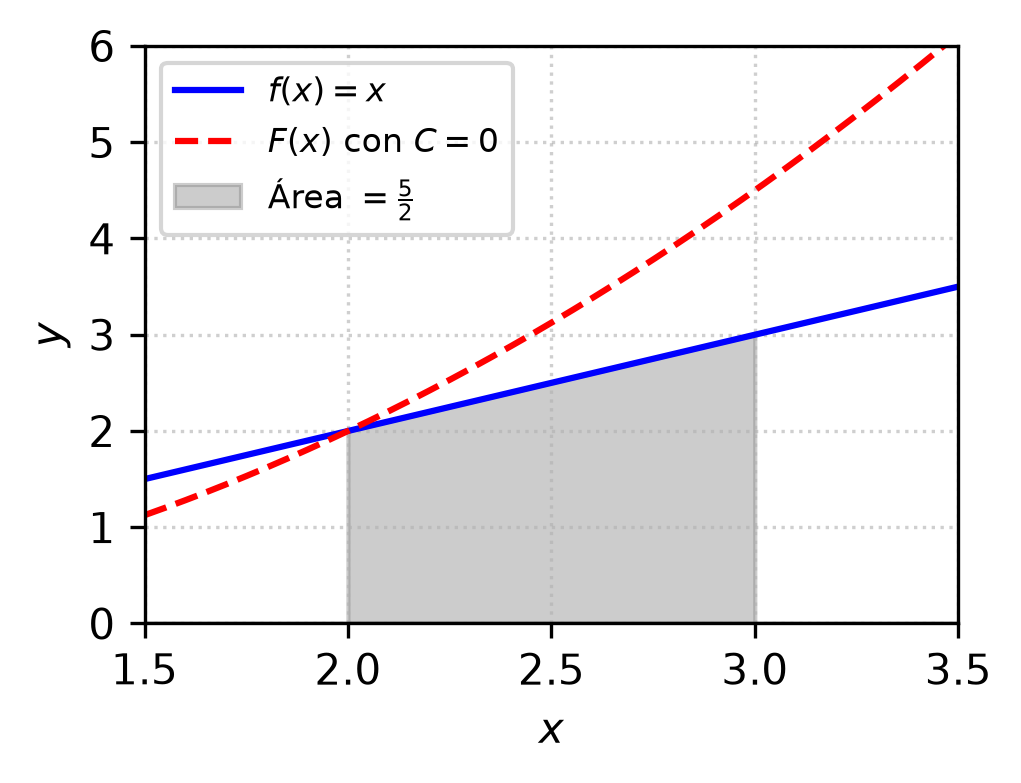
\includegraphics[width=\columnwidth]{semana_06/graficas/SEM06_P10_grafica.png}
	\caption{Representación gráfica de $f(x)$ y su antiderivada $F(x)$ evaluada para la constante de integración $C = 0$ (Problema 10).}
	\label{fig:problema10}
\end{figure}
